\section{ACCESORIOS Y CARACTERÍSTICAS}
\subsection{Palos de golf}
\begin{frame}{ACCESORIOS Y CARACTERÍSTCAS}
\framesubtitle{Palos de golf: maderas}
	Son los palos con los que se puede golpear más fuertemente y lograr mayor distancia.
	\begin{figure}[H]
      \centering
      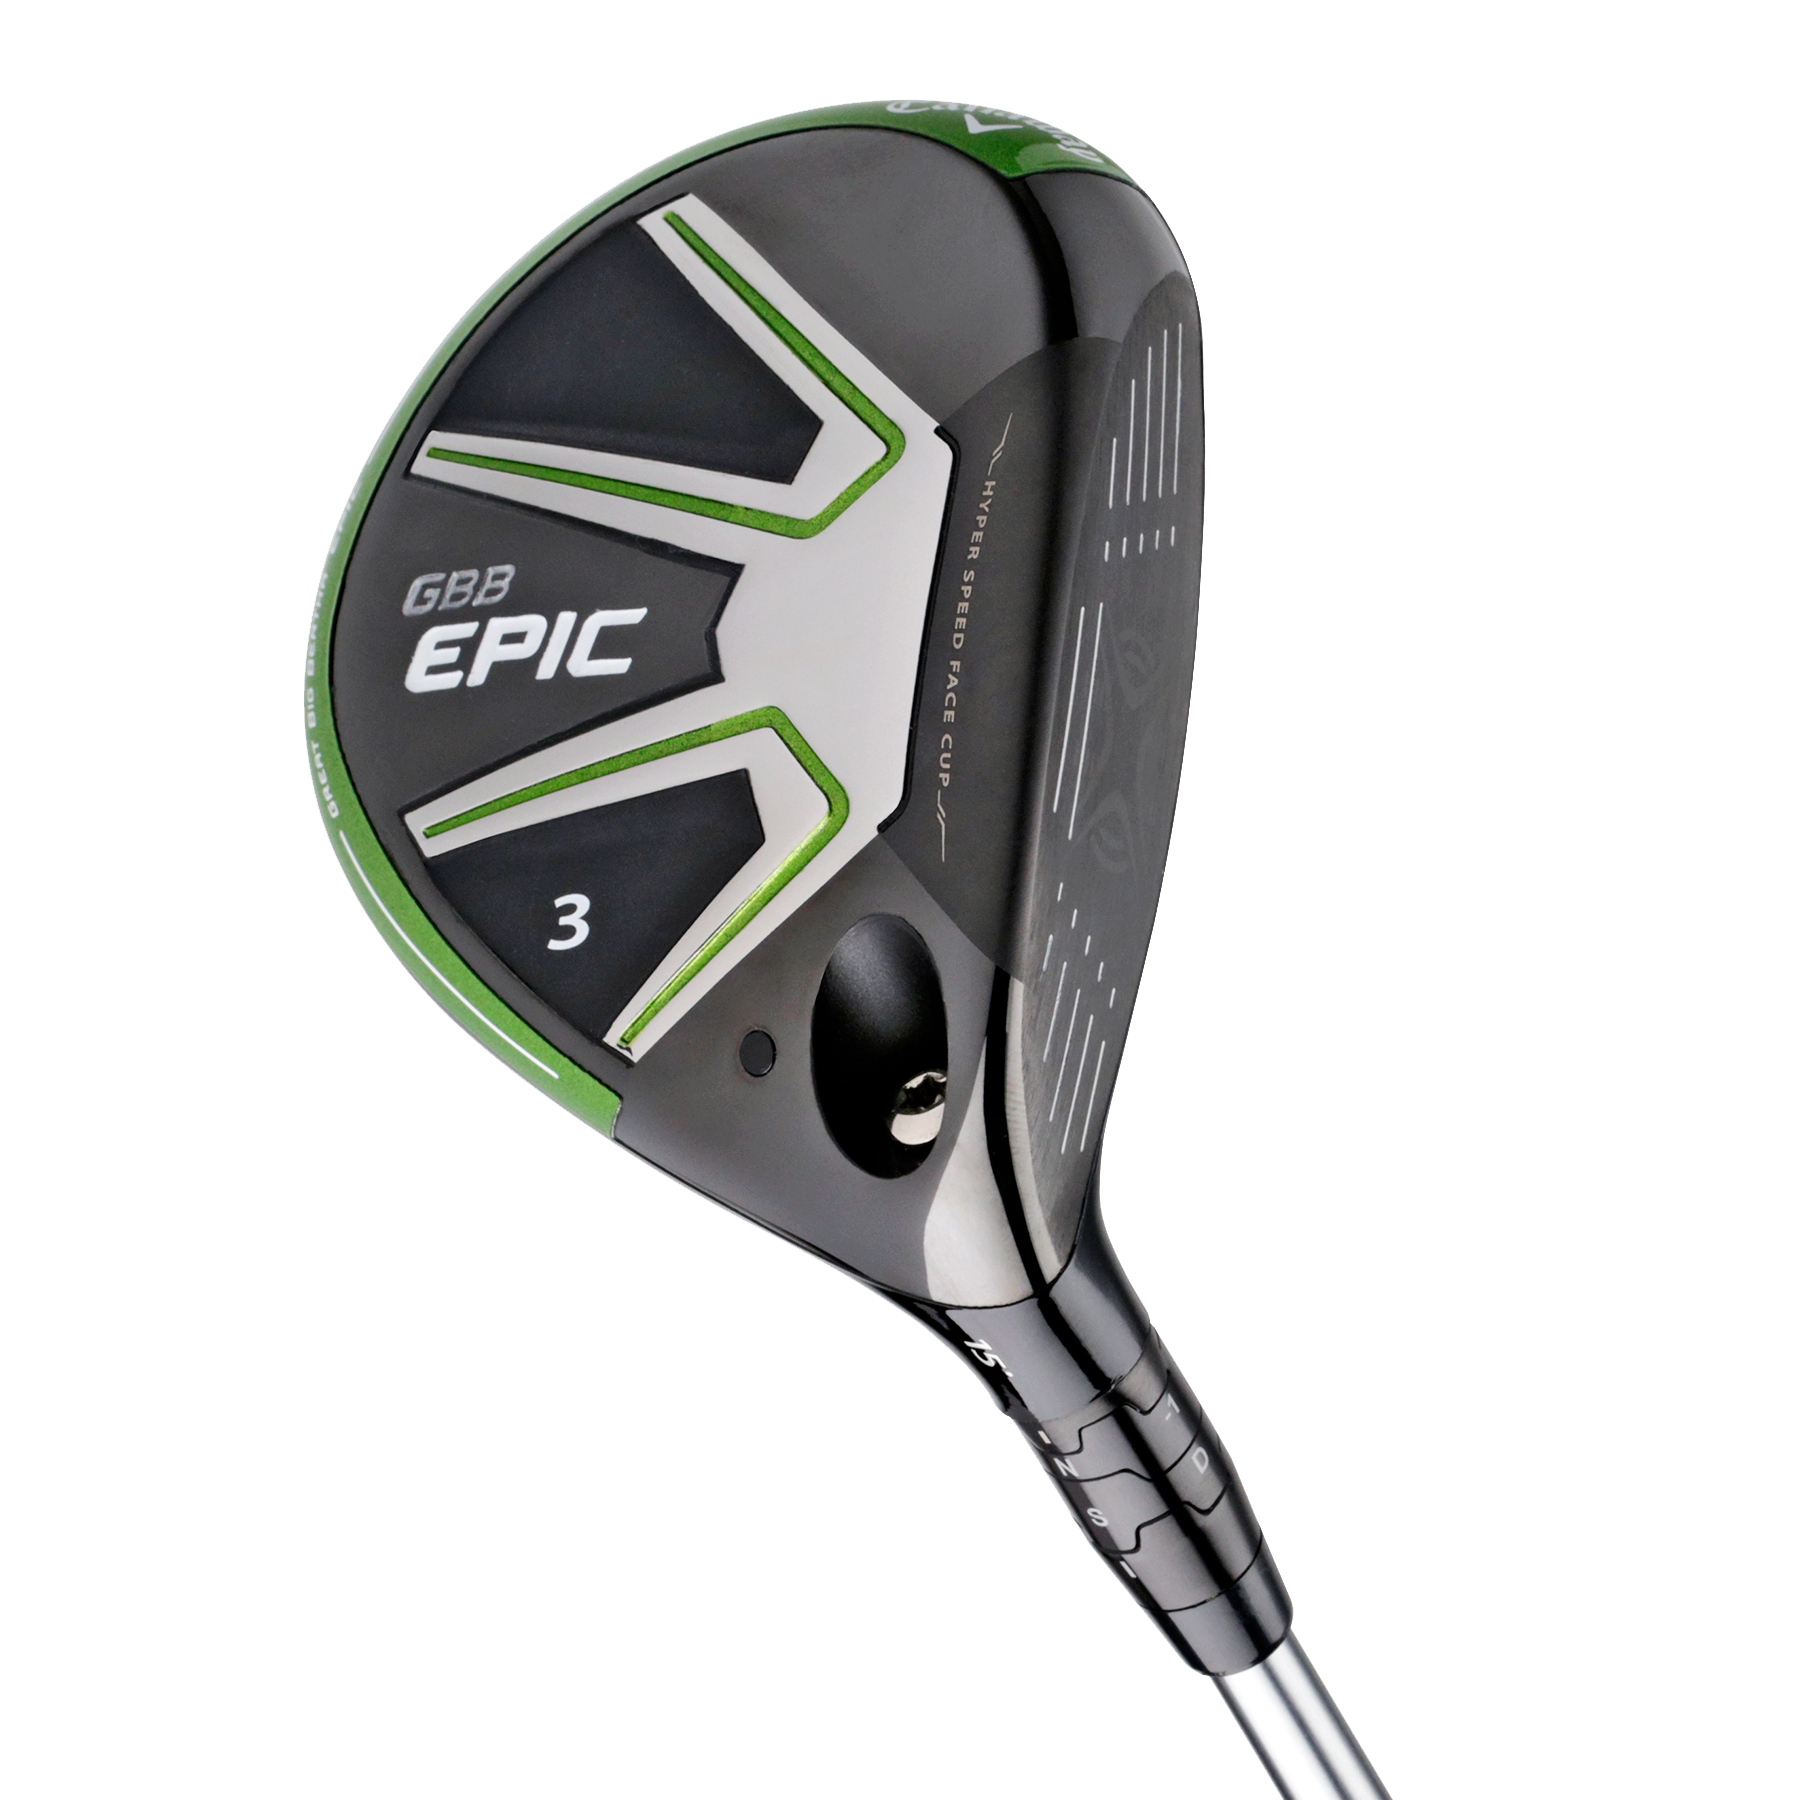
\includegraphics[scale = 0.075]{woods.png}
      \caption{Palo madera\footnotemark{}.}
	\end{figure}
    \footnotetext{\bibentry{woods}}
\end{frame}
%%%%%%%%%%%%%%%%%%%%%%
\begin{frame}{ACCESORIOS Y CARACTERÍSTICAS}
\framesubtitle{Palos de golf: wedge}
En éstos se consigue un mejor control de la bola, usualmente útil para situaciones difíciles.
	\begin{figure}[H]
      \centering
      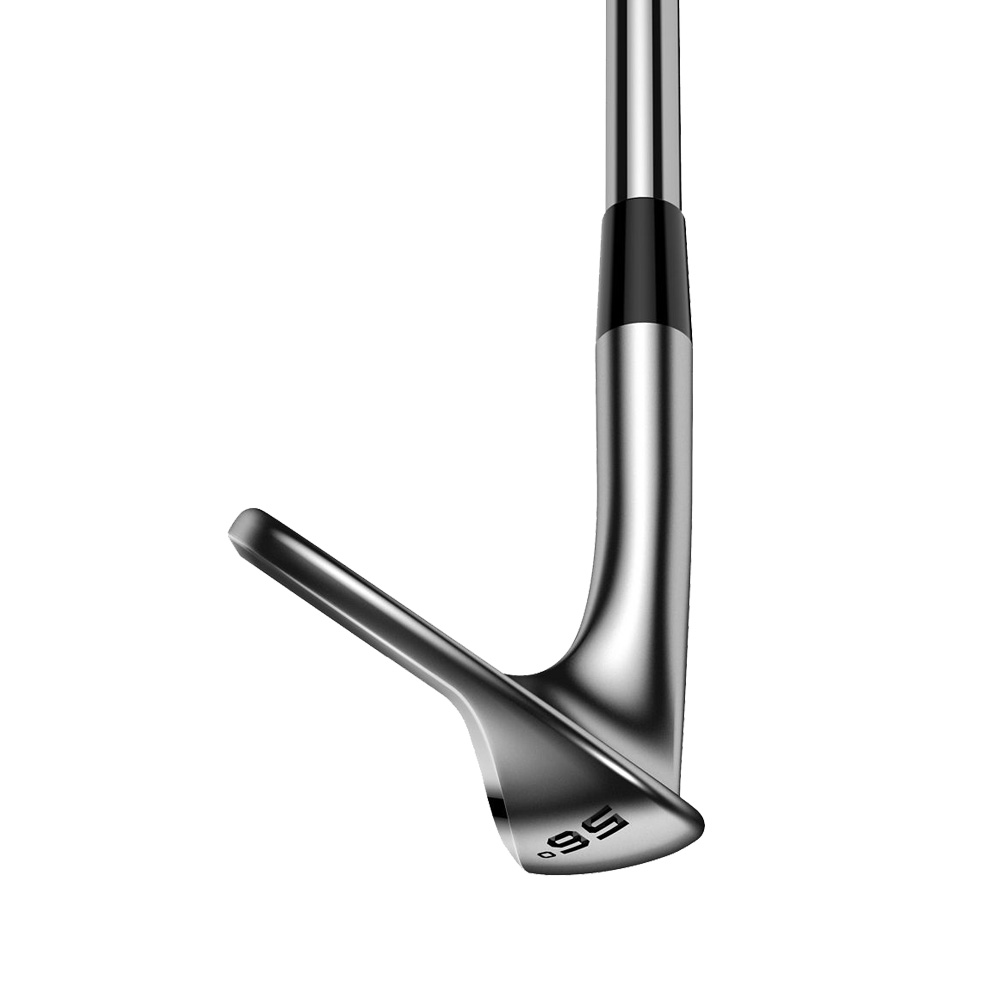
\includegraphics[scale = 0.125]{wedge.jpg}
      \caption{Palo wedge/iron\footnotemark{}.}
	\end{figure}
\vspace{-2cm}\footnotetext{\bibentry{wedge}}
\end{frame}

%%%%%%%%%%%%%%%%%%%%%%%
\begin{frame}{ACCESORIOS Y CARACTERÍSTICAS}
\framesubtitle{Palos de golf: putter}
Finalmente se utiliza un palo denominado putter para empujar la bola mediante un golpe (putt) hacia el hoyo en el green.
	\begin{figure}[H]
      \centering
      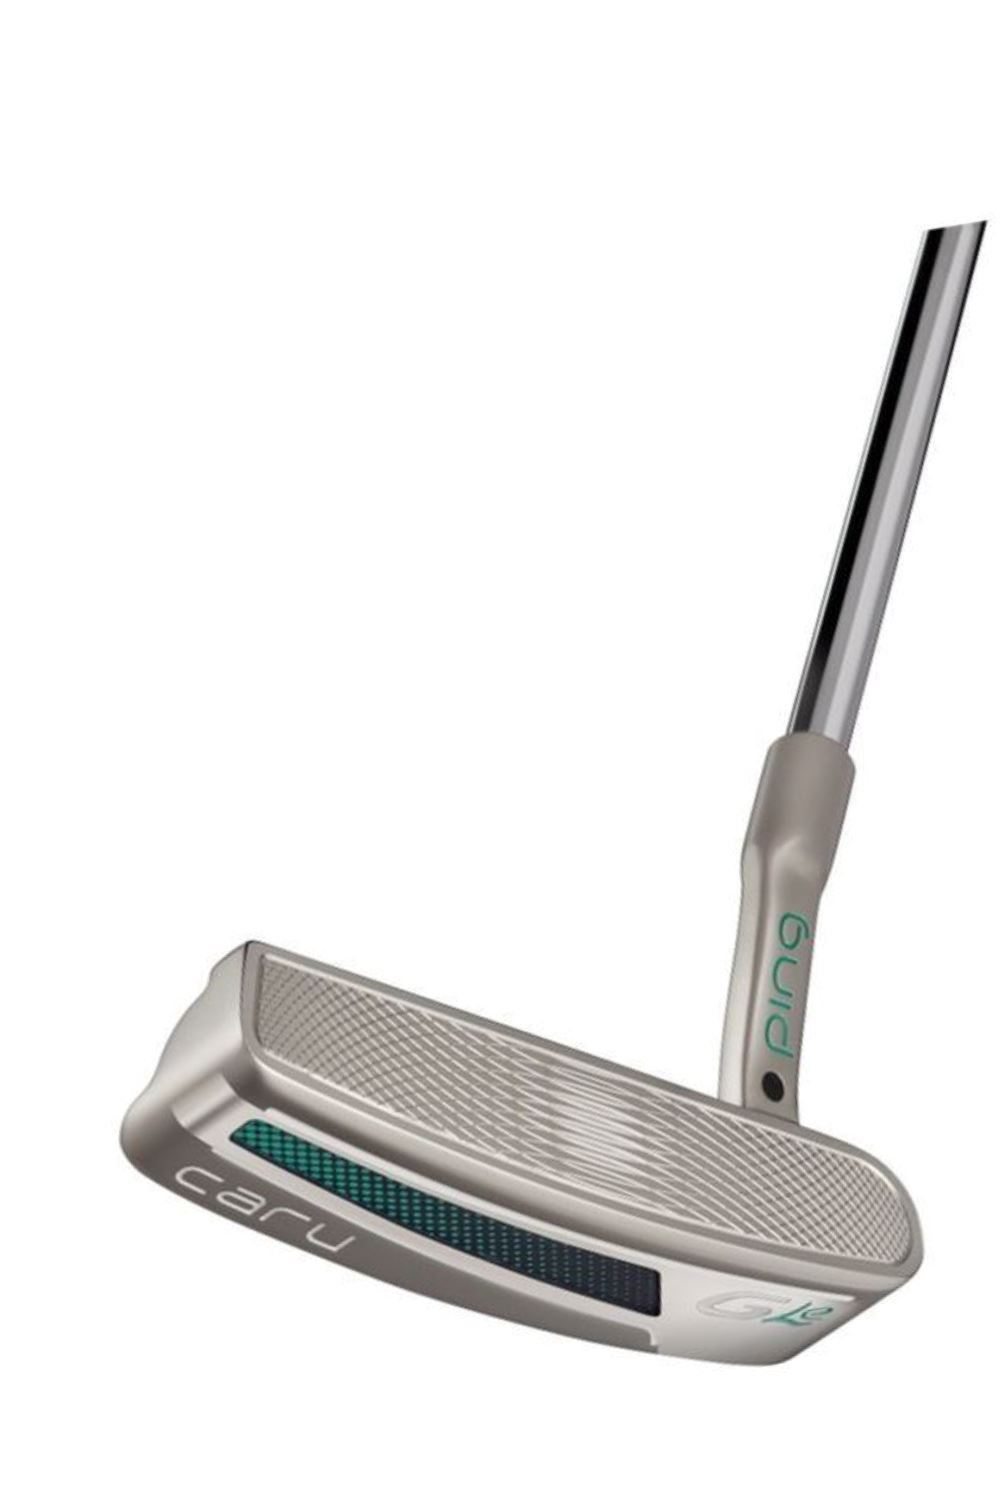
\includegraphics[scale = 0.125]{putter.jpeg}
      \caption{Palo putter\footnotemark{}.}
	\end{figure}
	\vspace{-1cm}\footnotetext{\bibentry{putter}}
\end{frame}
